% !TeX root = ../main.tex

\chapter{阴影感知的光照表示研究}

本文第3章通过混合的几何表示以及MLP纹理,实现了能够对数字资产进行指定工作流分解的管线。
虽然实验能够证明管线的适用性,但是部分定量实验以及定性实验的结果显示,管线无法处理明显的阴影关系,
导致阴影中的几何形状和反射属性的分解效果较差。
以Metallic工作流为例,该工作流的分解结果如图\ref{fig:shadow_error}所示。
在\ref{fig:shadow_albedo}Albedo分解输出中,阴影被错误地处理为场景表面固有的颜色;
而在\ref{fig:shadow_mesh}网格体分解输出中,阴影影响了管线对几何结构的判断。
同样,在其它对NeRF进行光照分解的研究中\cite{Zhang_2021, Wu_2023},
也存在阴影处的数据无法正确处理的问题。

\begin{figure}[H]
  \centering
  % 这里可以控制图片宽度比例
  \begin{subfigure}[t]{0.3\textwidth}
    \centering
    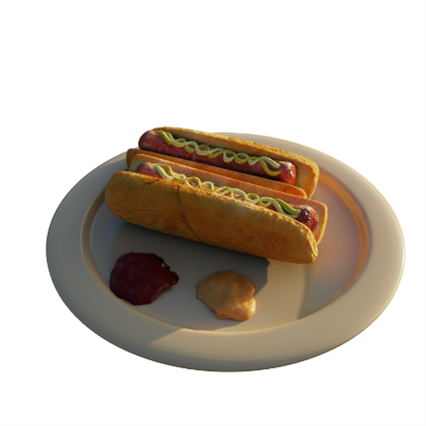
\includegraphics[width=\linewidth]{ch4/compare_in_shadow/shadow_gt.png}
    \caption{GT}
    \label{fig:shadow_gt}
  \end{subfigure}
  \begin{subfigure}[t]{0.3\textwidth}
    \centering
    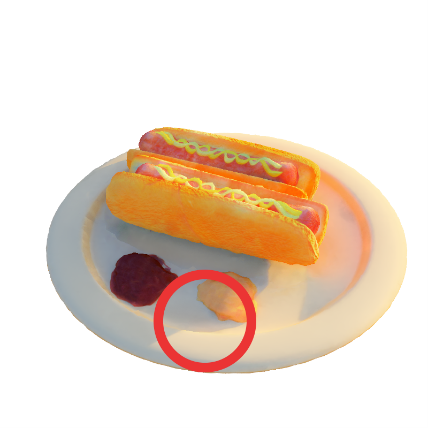
\includegraphics[width=\linewidth]{ch4/compare_in_shadow/shadow_albedo.png}
    \caption{Albedo分解输出}
    \label{fig:shadow_albedo}
  \end{subfigure}
  \begin{subfigure}[t]{0.3\textwidth}
    \centering
    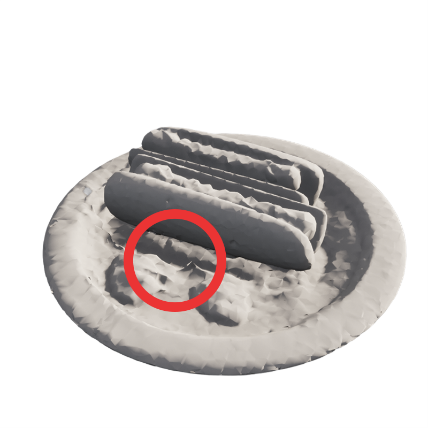
\includegraphics[width=\linewidth]{ch4/compare_in_shadow/shadow_mesh.png}
    \caption{网格体分解输出}
    \label{fig:shadow_mesh}
  \end{subfigure}
  \caption{阴影处分解效果对比}
  \label{fig:shadow_error}
\end{figure}

结合第3章实验结果及其它研究,这种错误可能来自于光照表示方法的不足。因此本章将改进光照表示方法,
以解决这一问题。接下来,本章首先将详细分析现有光照技术的表示能力,随后介绍本文提出的新颖光照表示方法。

\section{光照表示能力分析}

2.3.1介绍了IBL技术,该技术通过预滤波处理将半球积分转化为查表运算,实现了复杂全局光照的实时近似计算。
然而这种近似必然伴随物理真实性的折损:
其核心假设将\eqref{eq:rendering_equation}渲染方程中的入射光照
$L_i\left(\mathbf{x},\omega_i\right)$简化为$L(\omega_i)$,
本质上忽略了着色点空间位置$\mathbf{x}$对入射光$L_i$的影响。
这种降维处理导致IBL难以表示阴影等局部光照变化,如图\ref{fig:shadow_n_refl}所示,
当着色点位于反射方向$\omega_i$相近的平面时,不同空间位置$\mathbf{x}$的着色点可能因为阴影而接收到完全不同的入射光$L_i$。
因此,在传统的即时渲染器中,IBL技术通常仅被用作阴影处的光照补充,而阴影之外的着色点则通过其它离散形式的光源进行计算。

\begin{figure}[htb]
  \centering
  % 这里可以控制图片宽度比例
  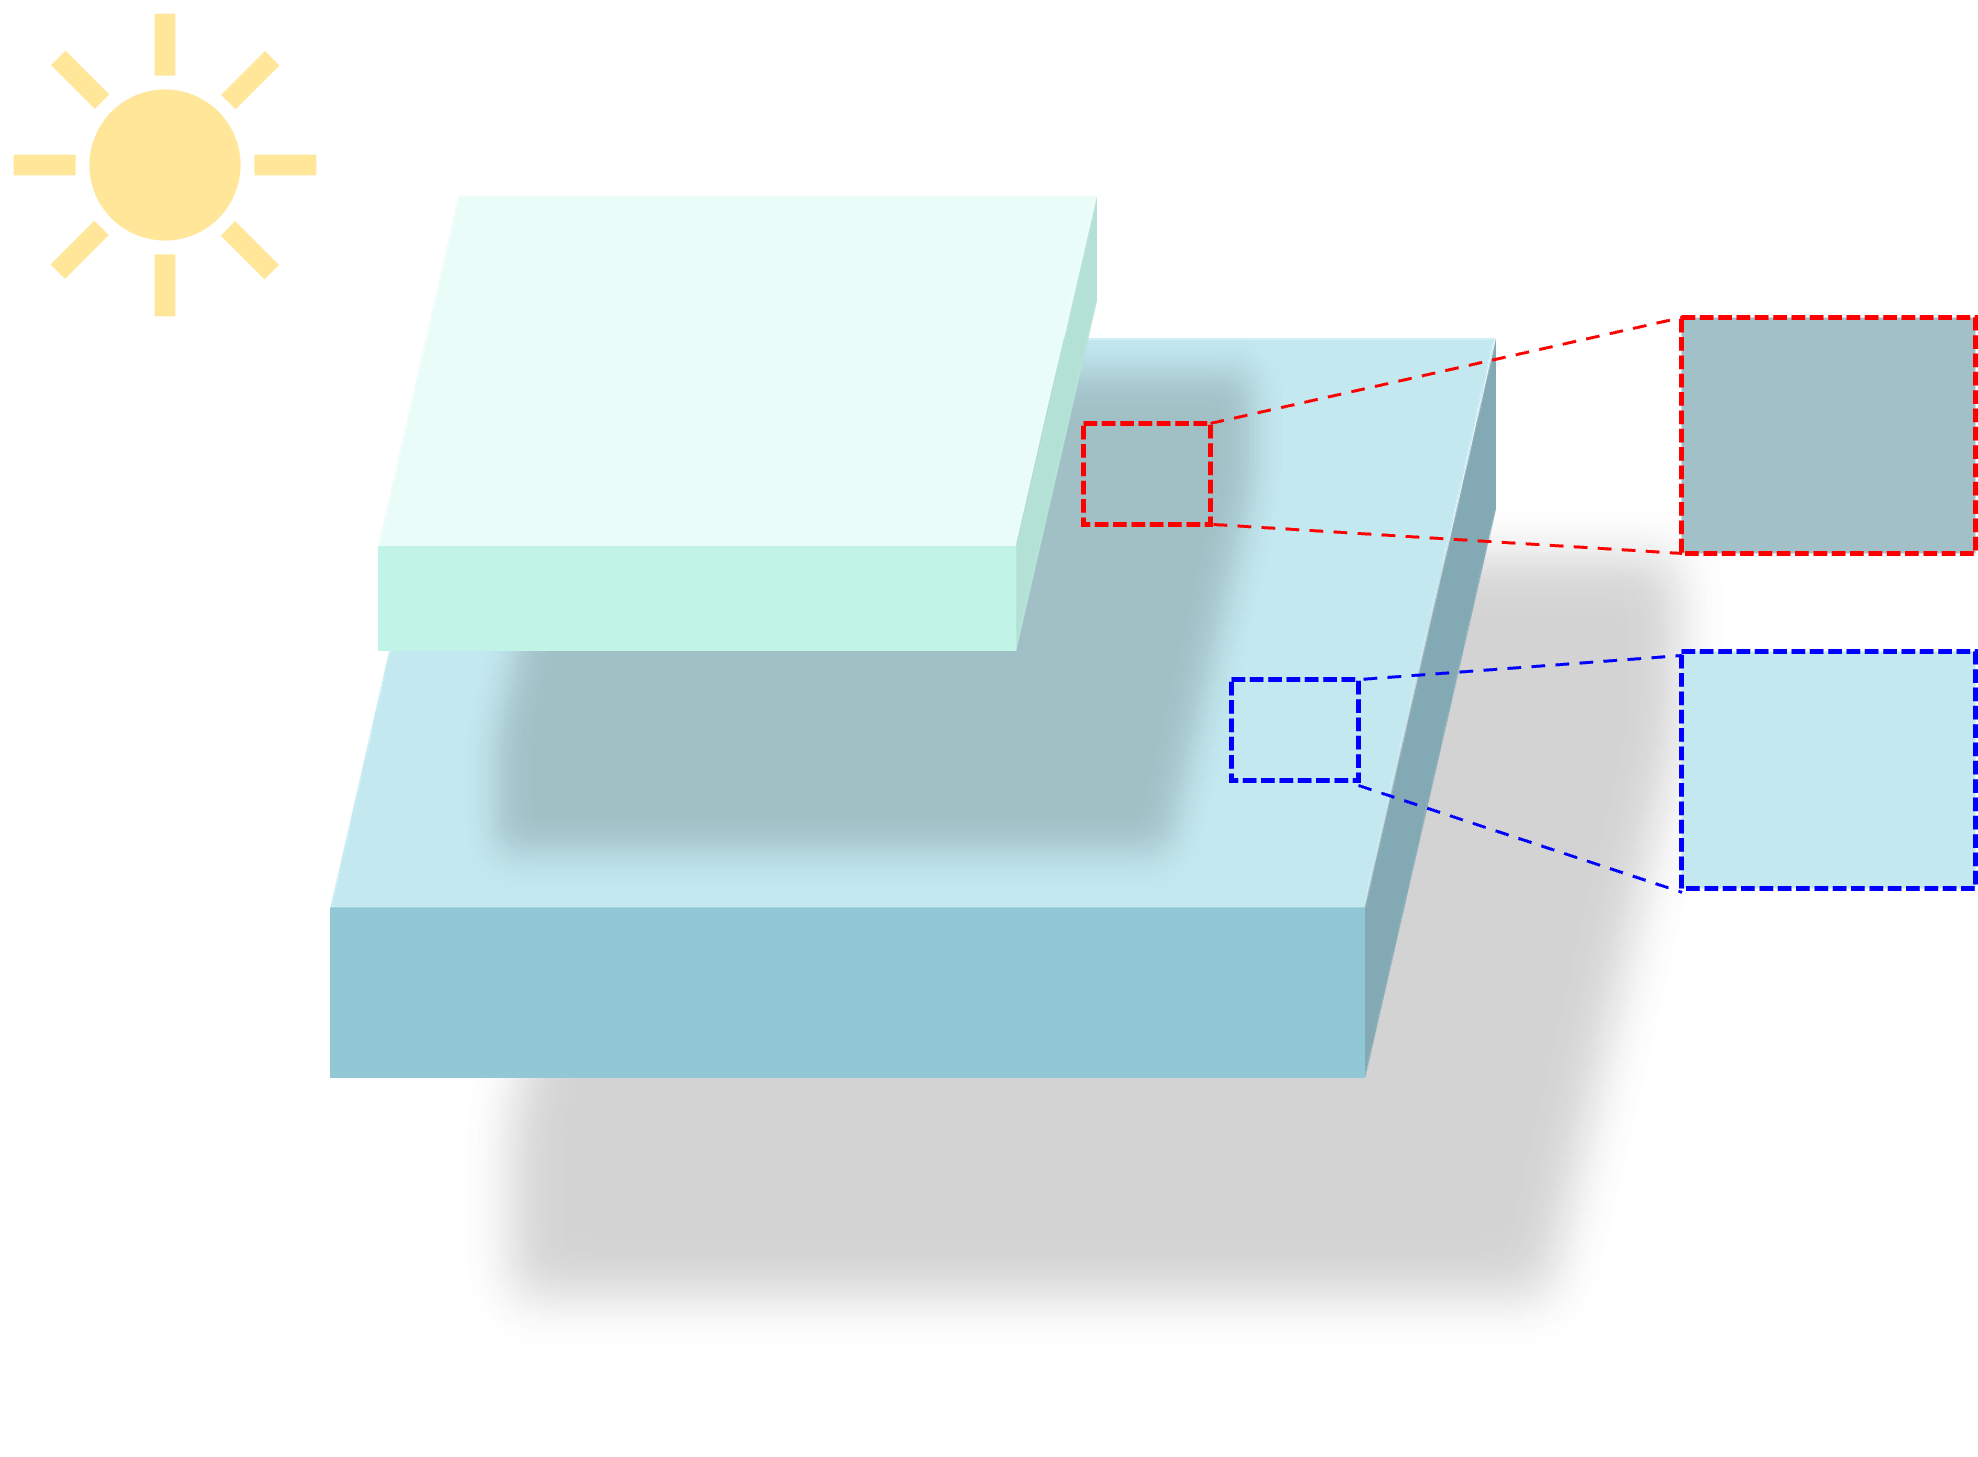
\includegraphics[width=0.8\linewidth]{ch4/shadow_n_refl.png}
  \caption{阴影对入射光照的影响}
  \label{fig:shadow_n_refl}
\end{figure}

为了改进这一点,本文考虑了上文所述的传统即时渲染中对IBL技术的应用方式,即仅将IBL作为完整光照的一部分补充,
用于增加阴影处的细节,记作环境光照$L_{env}$。而物体主要被直接光所照亮,记作$L_{direct}$。
本文中对直接光和环境光的分配可以由公式\eqref{eq:li_shadow}表示:

\begin{equation}
  \label{eq:li_shadow}
  L_i=\left(1-s\right)L_{\rm{direct}}+sL_{\rm{env}},
  \end{equation}

其中,$s$代表着色点处的阴影强度。该式反映出,直接光照的强度通常远高于环境光照,且只有直接光照能产生阴影,
而环境光照均匀地来自于一个球形的穹顶。因此,当着色点完全位于阴影之外时,环境光的贡献可以忽略,
直接光照主导;而当着色点进入阴影区域时,环境光的影响逐渐增加,成为主要的光照来源。
这种光照组合方式能够以较低的计算成本,显著提高阴影表示能力,同时几乎不增加优化的难度。
以上分析构成了本文创新的光照表示的基础,其并非对光照物理规律的完整数学描述,
而是将关键的物理原则嵌入到光照的组合方式中。这种策略在计算复杂度与光照表示能力之间取得了创新性平衡,
为后续的实现提供了清晰的框架。

\section{阴影调制模块与神经光照表示}

在上一节中,我们分析了IBL技术的局限性,并探讨了直接光和环境光的分配方式,
以进一步实现在较低的计算成本下增强光照表示能力的目标。基于以上分析,本文引入了神经光照表示方法,
以MLP为基础构建可学习的光照模型,从而扩展IBL在阴影场景中的适用性。

本节将介绍新颖的“阴影调制模块”,它能在神经网络的光照推理过程中引入对阴影的动态调控。
该模块不仅能捕捉局部阴影信息对光照分布的影响,还能与MLP主体紧密结合,从而在保持高效计算的同时,
大幅提升光照表示的准确度与逼真度。下面将详细阐述该模块的设计思路、实现细节以及它在神经光照表示框架中的作用。

\subsection{条件输入}

在机器学习中通常将基于上下文的处理称为条件:模型执行的计算会受到从辅助输入中提取的信息的制约或调节。
最简单的方法是将条件信息的表示与原有输入直接相连,将结果作为模型新的输入。该方法几乎不影响模型参数量,
但是条件信息会从输入层开始全部作用于后续的每一层。另一种方法是将条件信息与原输入相乘,条件信息可以对输入进行缩放,
以控制输入中哪些信息将进一步传递到后续的层。

Perez等人\cite{Perez_2018}将加法和乘积的方法结合,以仿射变换的形式将条件信息与输入结合,
称之为基于特征的线性变换(Feature-wise Linear Modulation,FiLM)。
仿射变换可以由公式\eqref{eq:film_affine}表示:
\begin{equation}
\label{eq:film_affine}
\varphi(x)=\gamma\cdot x+\beta
\end{equation}
其中,偏移量$\beta$和缩放系数$\gamma$被称为FiLM参数,仿射变换利用这些参数对输入$x$进行调制。

对于MLP来说,可以将特殊的FiLM层插入到模型中,以对该层的输入应用特征仿射变换。
FiLM参数(即偏移量$\beta$和缩放系数$\gamma$)由映射网络(Mappingnetwork)计算,
该网络利用条件信息$\mathbf{z}$作为输入,完成条件信息到FiLM参数的映射。
在这种设计下,虽然FiLM参数能够直接参与主网络的运算,但其实际为映射网络的输出结果,
因此FiLM参数不是传统意义上的具有固定权重的可学习参数,能够实现对主网络的调制。
FiLM层的计算方式如公式\eqref{eq:film_layer}所示,
\begin{equation}
\label{eq:film_layer}
\mathrm{FiLM}(\mathbf{x})=\gamma(\mathbf{z})\odot \mathbf{x}+\beta(\mathbf{z}).
\end{equation}
其中$\gamma(\mathbf{z})$和$\beta(\mathbf{z})$由映射网络计算,
$\odot$代表哈达玛乘积(Hadamard Product),对向量的各个分量之间逐个相乘。

本文则利用FiLM,将阴影视为条件输入至网络,利用FiLM调制阴影参数,以实现本文将阴影加入光照表示的目标。

\subsection{基于阴影调制模块的光照表示网络}

基于上述结构,本文设计了基于阴影调制模块的光照表示网络,其核心思想是将阴影系数$s$作为额外的标量参数调制到网络中。
当阴影系数为1时,在该模块的调制下,本文的网络将退化为一张环境光照贴图,其输出将全部为环境光照。
当阴影系数为0时,则使本文的网络输出为直接光照的光照强度及颜色。该网络的结构如\ref{fig:nl_main_cn}所示,
其接收入射光照的方向$\omega_i$作为输入,随后先调制阴影系数$s$,并在后续的层中逐步调制光照嵌入向量$\bf{z}^l$,
用以表示整张环境纹理。光照嵌入向量$\bf{z}^l$和阴影系数$s$的生成将在后文进一步介绍。

\begin{figure}[htb]
  \centering
  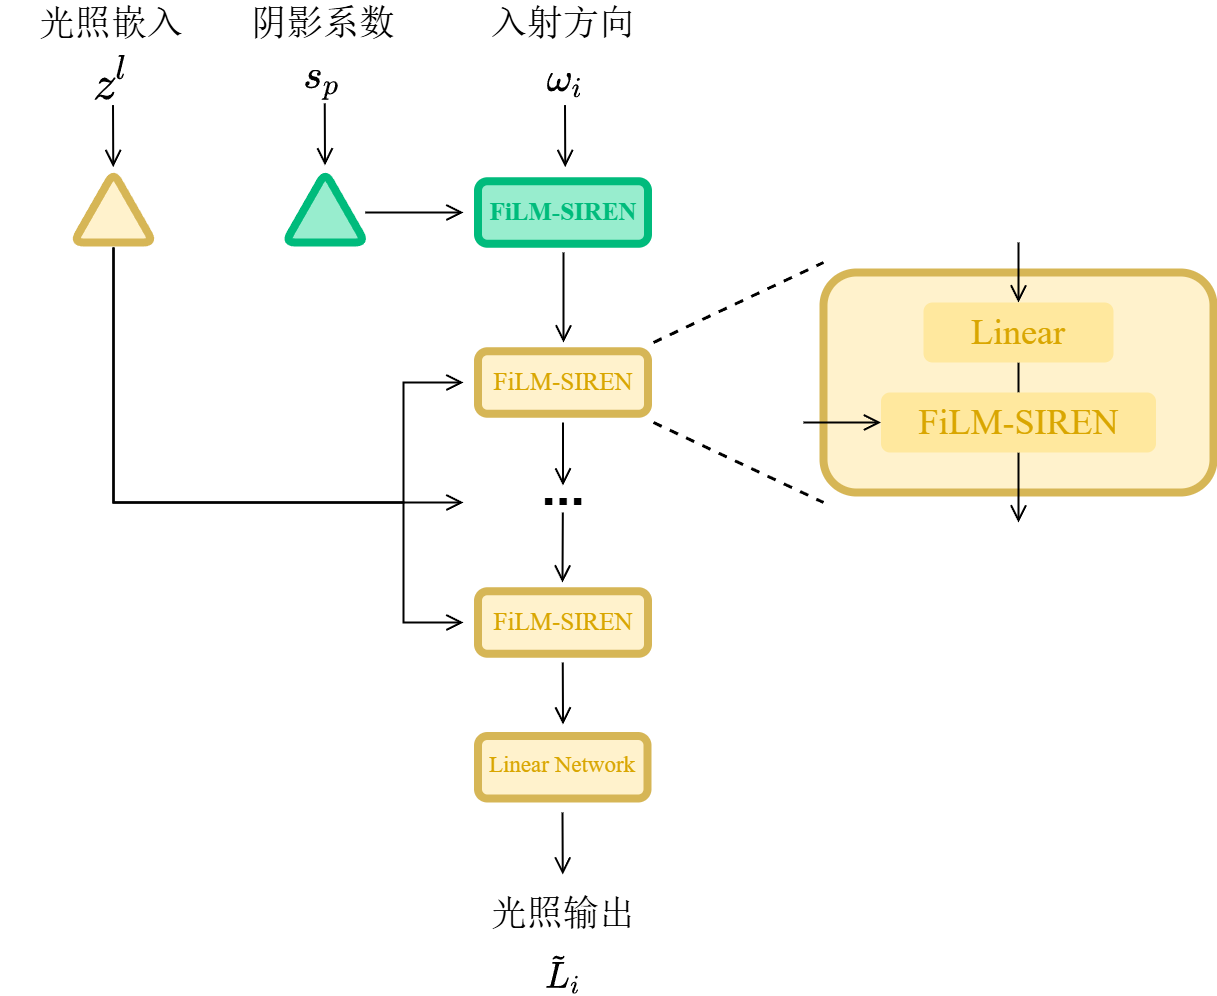
\includegraphics[width=0.6\linewidth]{ch4/nl_main_cn.png}
  \caption{光照表示网络结构图}
  \label{fig:nl_main_cn}
\end{figure}

对于映射网络,其结构如图\ref{fig:nl_main_cn}所示。该网络首先通过傅里叶编码将标量条件
输入映射到高维特征空间,从而提取出多频率的信息,增强了输入的表达能力。接着,转换后的特征被送入一个小型MLP,
该网络包含一个采用ELU激活函数的隐藏层,以捕捉输入数据的复杂特性;
随后,一个线性激活的全连接层进一步将特征映射到所需维度,并最终通过重塑操作生成参数对。

\begin{figure}[htb]
  \centering
  
\includegraphics[width=0.6\linewidth]{ch4/mapping_net.png}
  \caption{映射网络结构图}
  \label{fig:nl_main_cn}
\end{figure}

最终,该光照表示网络将会构建类似“体积”纹理的光照表示,如图\ref{fig:nl_light_volume}所示,其根据阴影系数来对直接光照和环境光照进行插值,
实现了对两种光照的统一编码。

\begin{figure}[htb]
  \centering
  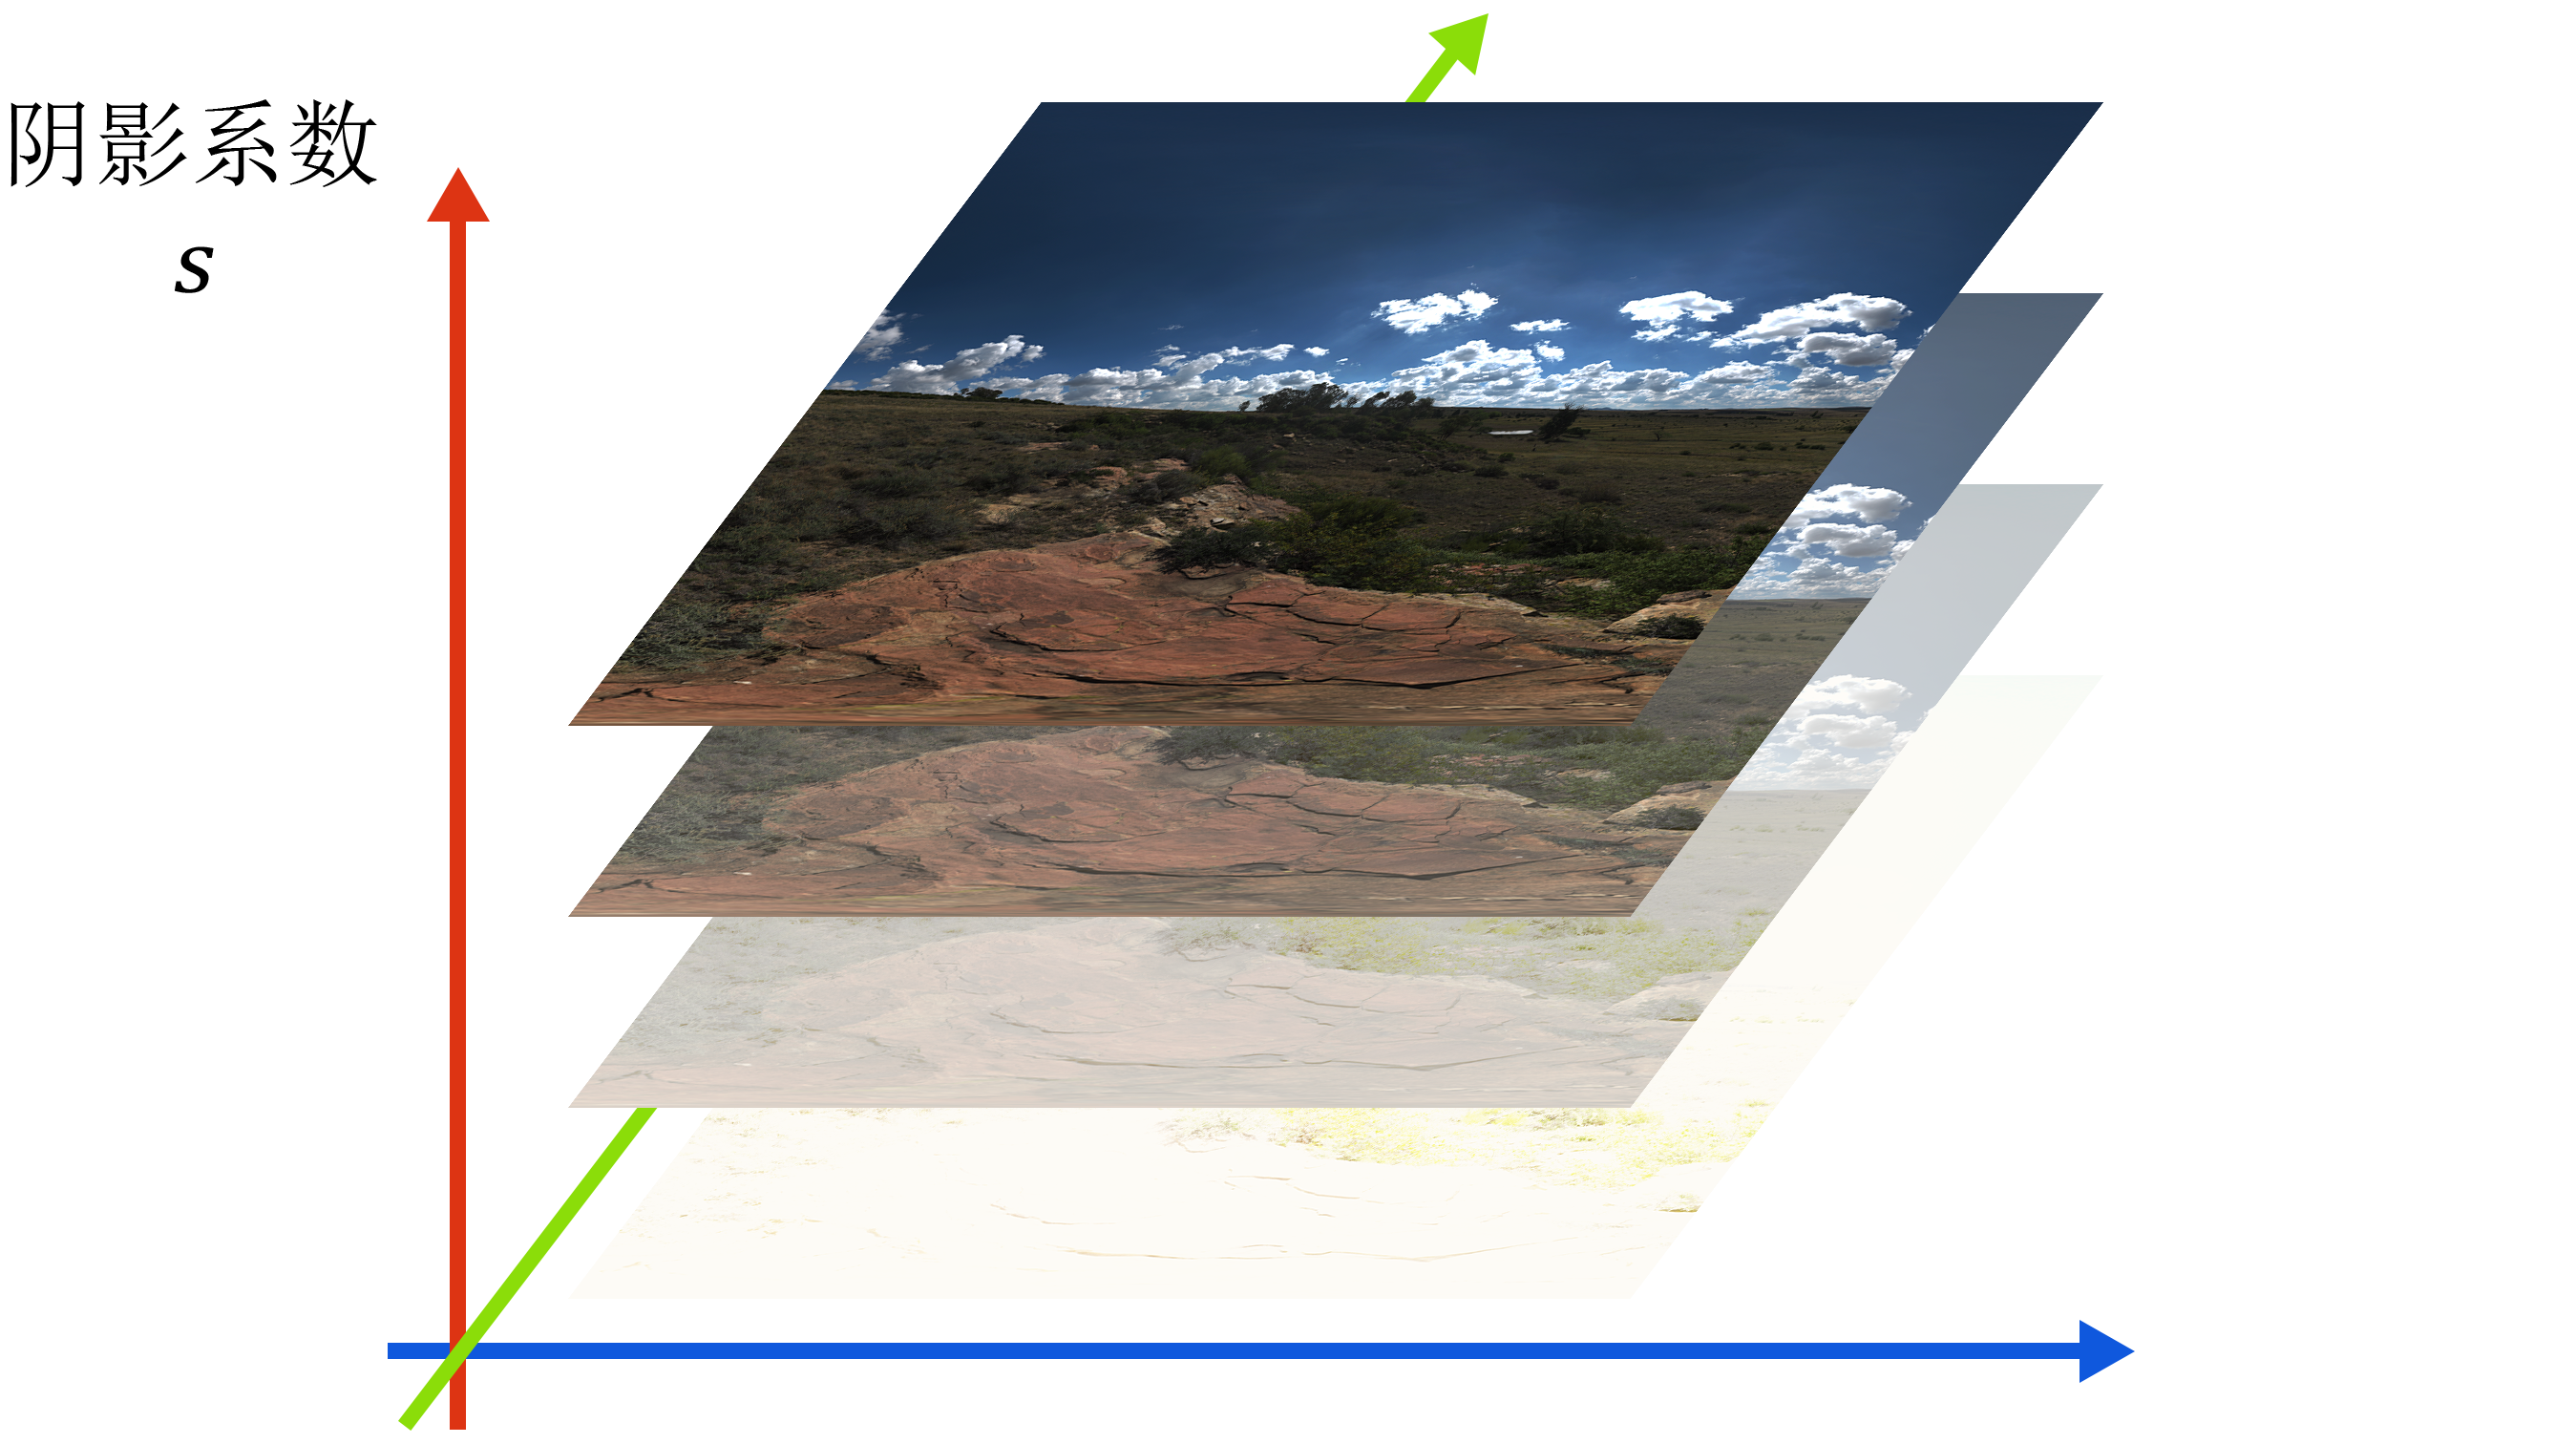
\includegraphics[width=0.6\linewidth]{ch4/sanl_light_show.png}
  \caption{网络光照关系示意图}
  \label{fig:nl_light_volume}
\end{figure}

\subsection{潜空间自动编码器}

对于上文提到的光照嵌入向量${\bf{z}}^l$,本文了参考Mark等人\cite{boss2021neural}的工作,通过自动编码器生成。
\ref{sec:auto_encoder}中介绍了自动编码器对于可微渲染的作用,Mark等人使用真实的环境纹理对自动编码器进行预训练,
该自动编码器能够将256$\times$256的环境纹理映射到128维向量,并使用多个损失函数约束潜空间,最终该自动编码器实现了
对具备真实感的光照潜空间,非常适合神经光照相关的任务。

该自动编码器通过四个损失函数的组合实现上述功能。首先是标准的重建损失$\mathcal{L}_{\mathcal{r}}$,可以通过以下公式定义:

\begin{equation}
  \label{eq:reconstruction_loss}
  \mathcal{L}_{\mathcal{r}}=\mathbb{C}_{E\sim\mathcal{D}_{\mathrm{light}}}\left[\|E-\mathcal{G}\left(\mathcal{E}(E)\right)\|_{\mathrm{Frobenius}}^2\right].
  \end{equation}
  其中$E$为编码器,$\mathcal{G}$为解码器,通过Frobenius范数保持像素级一致性。
  
  随后是循环一致损失$\mathcal{L}_{\mathcal{c}}$,该损失可以强制解码器的输出来自于编码器输入中的特征,其表达式为:
  \begin{equation}
  \label{eq:cycle_loss}
  \mathcal{L}_{\mathcal{c}}=\frac{1}{m}\sum_{n=1}^{m}\left|z_n'-\mathcal{E}\left(\mathcal{G}\left(z_n'\right)\right)\right|_{\Sigma^{-1}}^2.
  \end{equation}
  
  其次,为了使得潜空间向量$\mathcal{G}\left(z'\right)$生成的数据具备物理真实感,
  能够服从真实的光照分布,该自动编码器通过辨别器网络引入了对抗损失$\mathcal{L}_{\mathcal{a}}$:
  \begin{equation}
  \label{eq:adversarial_loss}
  \mathcal{L}_{\mathcal{a}}=\mathbb{C}_{z_a,z_b}\left[\|\mathcal{D}\left(\mathcal{G}\left(z'\right)\right)-1\|_2^2\right]+\mathbb{C}_E\left[\|\mathcal{D}\left(E\right)\|_2^2\right].
  \end{equation}
  这确保了插值的潜空间向量$\mathcal{G}\left(z'\right)$可以生成合理的数据,使得结果服从真实的光照分布,更具真实感。
  
  最后,该编码器使用曲率正则化$\mathcal{L}_{\mathcal{s}}$损失以确保流形局部平坦,
  避免生成的光照数据发生突变或空洞,其表达式为:
  \begin{equation}
  \label{eq:curvature_loss}
  \mathcal{L}_{\mathcal{s}}=\mathbb{C}_{\alpha\sim U\left(\mathbb{0},\mathbb{1}\right)}\left[\|J_{\mathcal{G}}\bigl(z(\alpha)\bigr)\cdot\frac{\partial z}{\partial\alpha}\|_{\mathrm{HS}}^2\right],
  \end{equation}
  其中$J_{\mathcal{G}}$为解码器的Jacobian矩阵,通过Hilbert-Schmidt范数惩罚路径曲率。
  
  最终的损失$\mathcal{L}$为上述四个损失的加权和,表达式为:
  \begin{equation}
  \label{eq:total_loss}
  \mathcal{L}=\mathcal{L}_{\mathcal{r}}+\lambda_1\mathcal{L}_{\mathcal{c}}+\lambda_2\mathcal{L}_{\mathcal{a}}+\lambda_3\mathcal{L}_{\mathcal{s}}.
\end{equation}

\section{数据集的获取}

由于本文希望SaNL能够学习到阴影与环境光照之间的关系,因此相较于其它的神经网络,
SaNL需要收集额外的数据集。根据前文的设计,SaNL需要入射光线方向$\omega_i$、阴影系数$s$、光照嵌入$z_l$作为输入数据,
以及入射光照$L_i$作为监督信号。本文通过渲染引擎收集了多组包含上述数据的合成数据集,下面介绍收集该数据集的方法及过程。

\section{入射光线方向数据}

在先前的研究中,入射光线方向$\omega_i$通常在训练时随机生成,不在数据集内提供。
本文考虑到入射光线方向与场景的几何形状直接相关,而IBL技术中,相似的几何形状可能在环境贴图中采样的区域相近,
因此本文选择根据网格体来收集真实的场景几何形状。为了增强数据集的多样性,在选择网格体时应充分考虑包括不同的几何结构。
同时,为了方便收集阴影系数数据,网格体也应有丰富的自遮挡。

本文选取的8个网格体如图\ref{fig:data_mesh}所示。这些网格体形状各异,如Sofa、Car等网格体具有细微尖锐的高频细节,
Teapot、Statue有平滑圆润的表面,而Beach、Girl的几何结构则能生成充分的自阴影。

\begin{figure}[htbp]
  \centering
  \renewcommand{\arraystretch}{1} % 调整表格行距
  \setlength{\tabcolsep}{3pt} % 调整列间距

  \begin{tabular}{c c c c}
      \subfloat{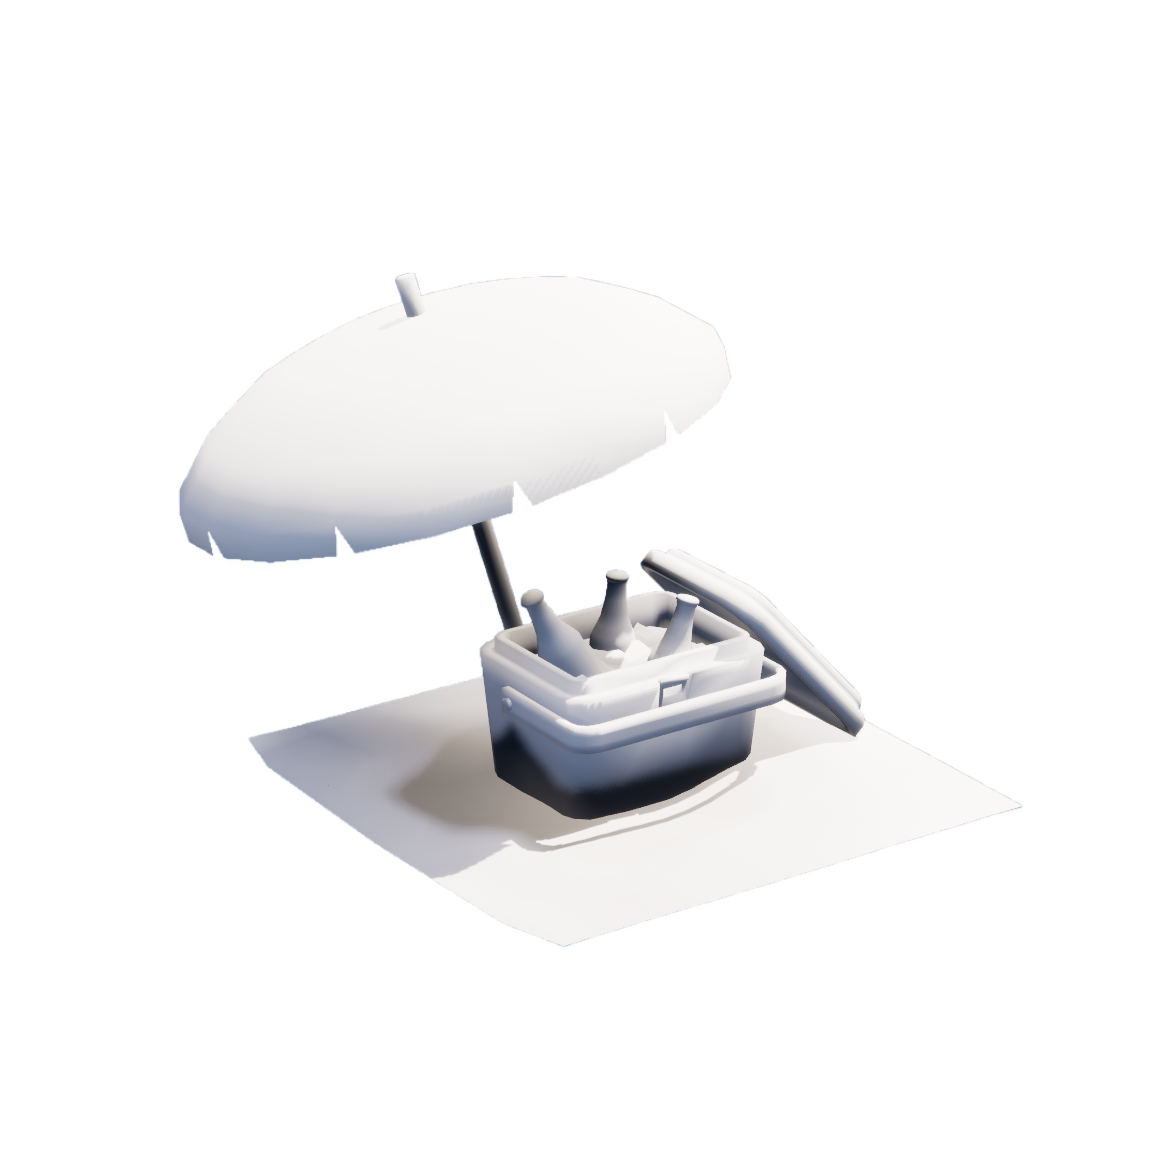
\includegraphics[width=0.22\textwidth]{ch4/sanl_data_mesh/beach.png}} &
      \subfloat{\includegraphics[width=0.22\textwidth]{ch4/sanl_data_mesh/Girl.png}} &
      \subfloat{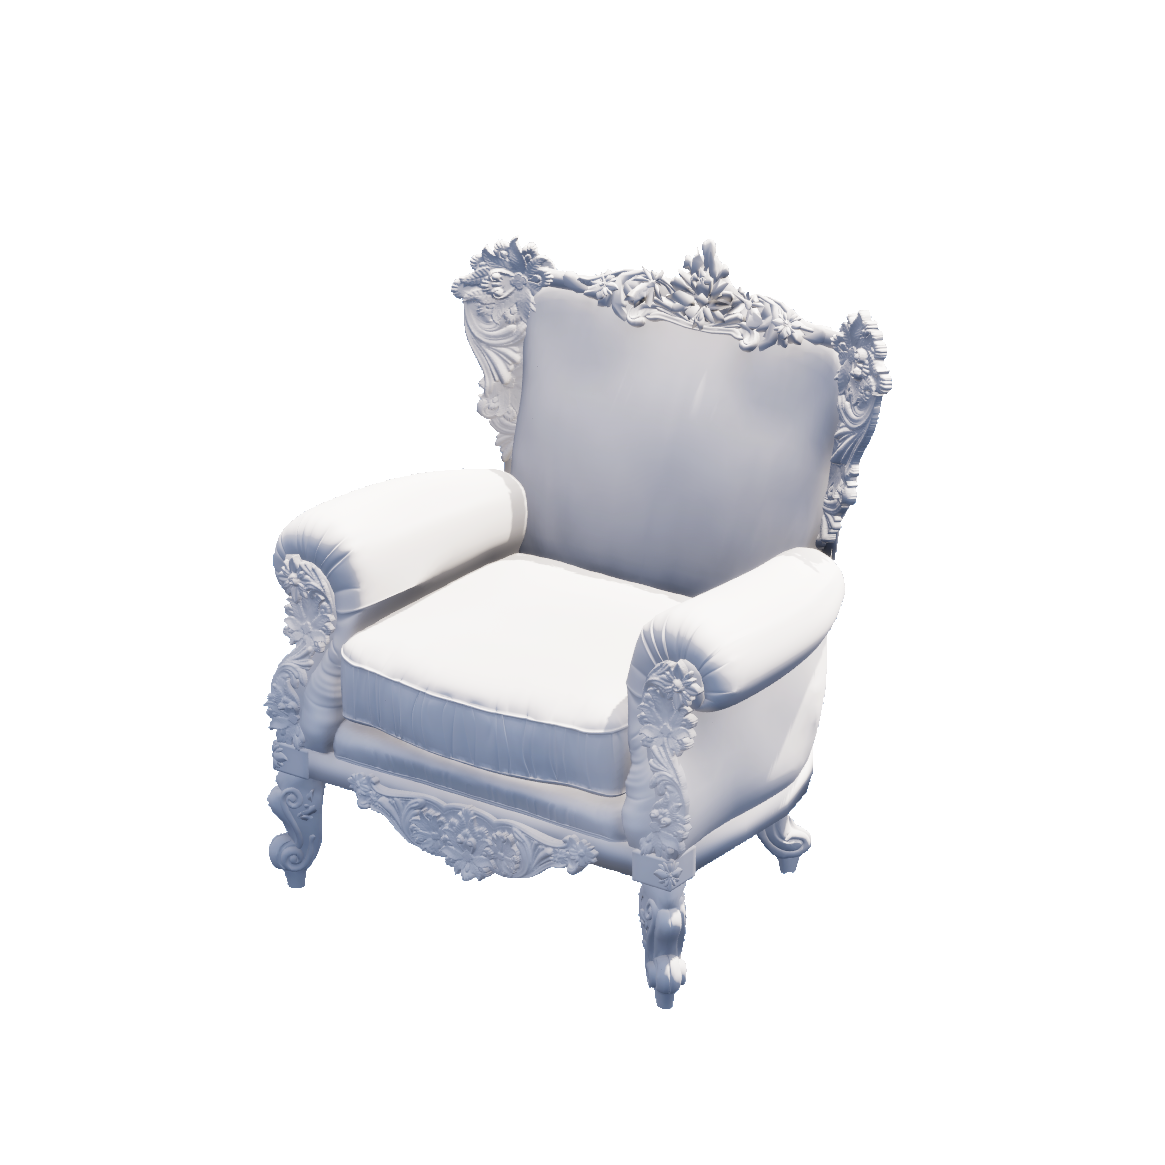
\includegraphics[width=0.22\textwidth]{ch4/sanl_data_mesh/chair.png}} &
      \subfloat{\includegraphics[width=0.22\textwidth]{ch4/sanl_data_mesh/Car.png}} \\
      Beach & Girl & Sofa & Car\\

      \subfloat{\includegraphics[width=0.22\textwidth]{ch4/sanl_data_mesh/Rabbit.png}} &
      \subfloat{\includegraphics[width=0.22\textwidth]{ch4/sanl_data_mesh/Skull.png}} &
      \subfloat{\includegraphics[width=0.22\textwidth]{ch4/sanl_data_mesh/Teapot.png}} &
      \subfloat{\includegraphics[width=0.22\textwidth]{ch4/sanl_data_mesh/Statue.png}} \\
      Rabbit & Skull & Teapot & Statue\\
  \end{tabular}

  \caption{构成数据集的网格体}
  \label{fig:data_mesh}
\end{figure}

\subsection{光照与阴影数据}

入射光照数据$L_i$作为SaNL的监督信号,需要充分考虑直接光照和环境光照的关系。对于环境光照,
本文使用了500张高质量的HDR立方体纹理作为环境光照的数据来源,这些立方体纹理将以IBL技术向场景内投射光照,
同时,为了获得更加多样的环境光照数据,这些立方体纹理会围绕$Z$轴随机旋转,尽可能地记录纹理中不同区域的光照。

直接光照部分,本文使用单盏平行光模拟,随机生成光照方向。为了使直接光照更符合真实情况,
直接光照的仰角随机范围为[15, 85]之间,方位角范围为[0, 360]之间。同时,为了增加网络对不同颜色的直接光照的泛化性,
本文使用色温描述直接光照颜色,随机范围为[5000, 10000]开尔文。阴影数据$s$也同样由该盏直接光照在网格体上照射产生。
直接光照和环境光照将按照公式\eqref{eq:li_shadow}进行插值,并输出为监督信号$L_i$。

对于光照嵌入向量$z_l$,需要一张环境纹理$I$作为自动编码器进行计算,因此本文将上述环境光照和直接光照烘焙至
一张新的HDR立方体贴图,分辨率为$128\times128\times6$。这种烘焙的策略能使得光照嵌入向量$z_l$不仅保留了环境光照的信息,
还加入了直接光照的亮度、色温、方向等信息。烘焙前后的对比如图所示。

\begin{figure}[H]
  \centering
  % 这里可以控制图片宽度比例
  \begin{subfigure}[t]{0.45\textwidth}
    \centering
    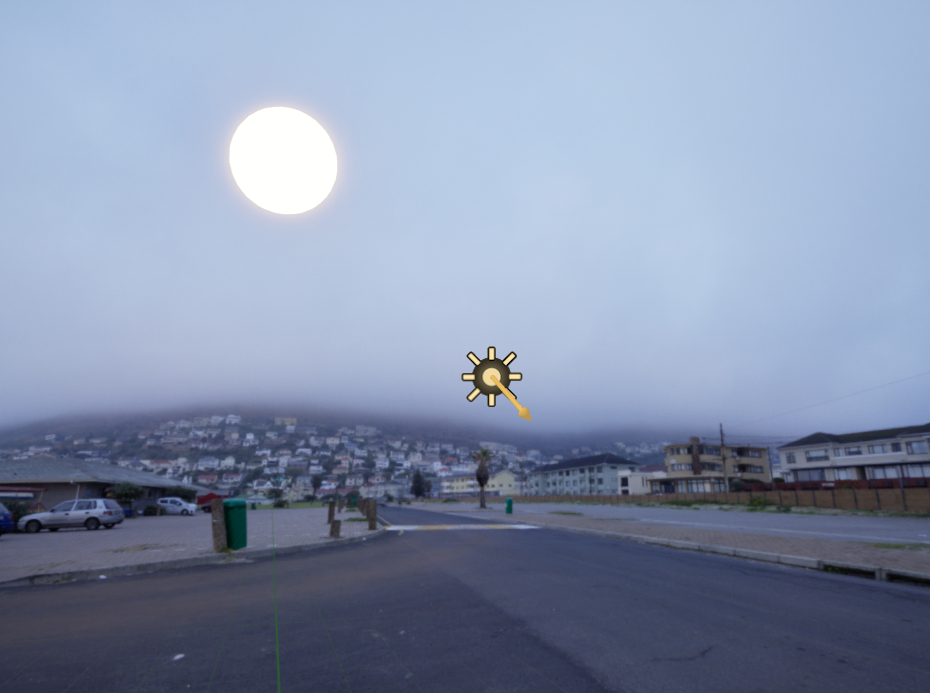
\includegraphics[width=\linewidth]{ch4/data_set/before.png}
    \caption{烘焙前}
  \end{subfigure}
  \begin{subfigure}[t]{0.45\textwidth}
    \centering
    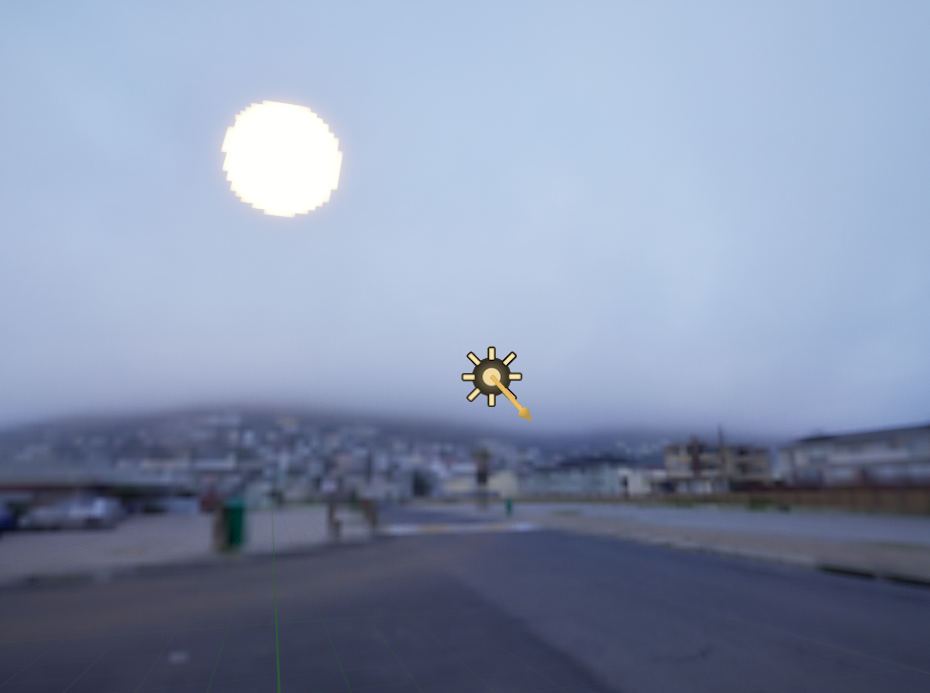
\includegraphics[width=\linewidth]{ch4/data_set/after.png}
    \caption{烘焙后}
  \end{subfigure}
  \caption{环境光照与直接光照烘焙}
  \label{fig:light_baking}
\end{figure}

最终,完整的数据收集过程如图\ref{fig:full_pipe}所示。

\begin{figure}[htb]
  \centering
  % 这里可以控制图片宽度比例
  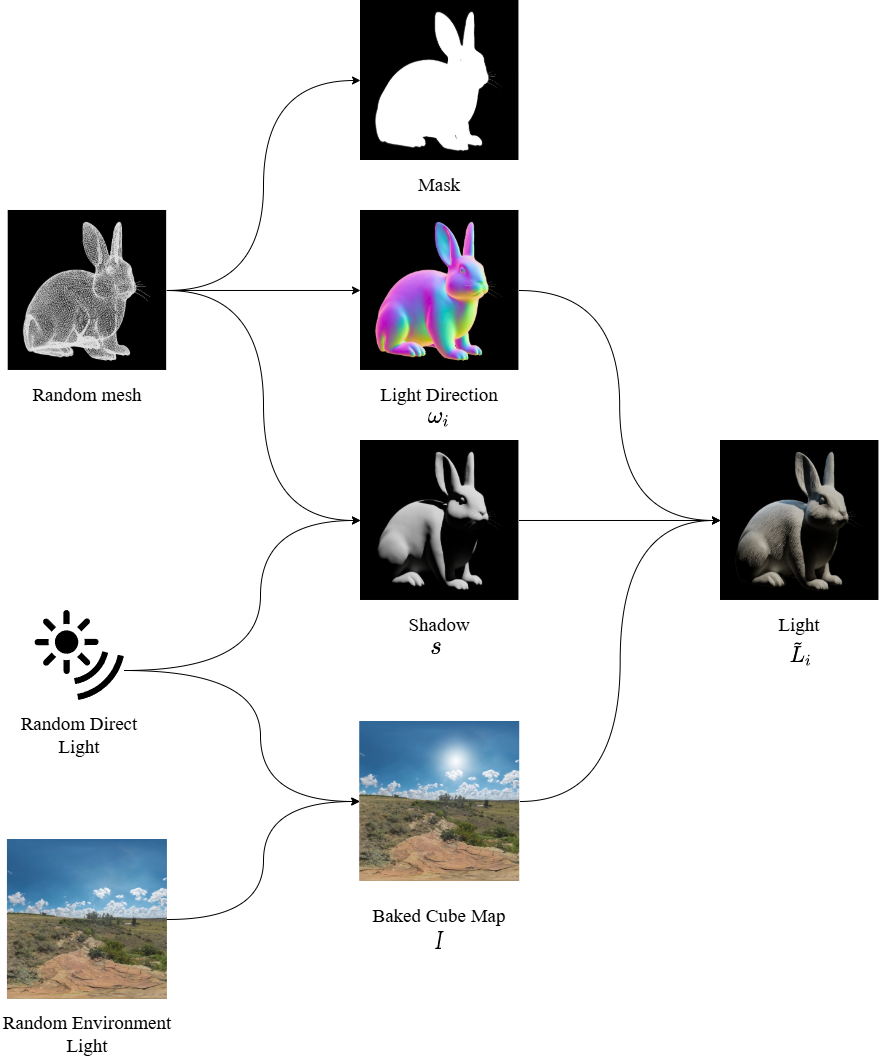
\includegraphics[width=0.8\linewidth]{ch4/data_set/full_pipe.png}
  \caption{数据集完整收集流程}
  \label{fig:full_pipe}
\end{figure}